Consider the following system.  Box and label your answers to each of the parts.
\begin{center}
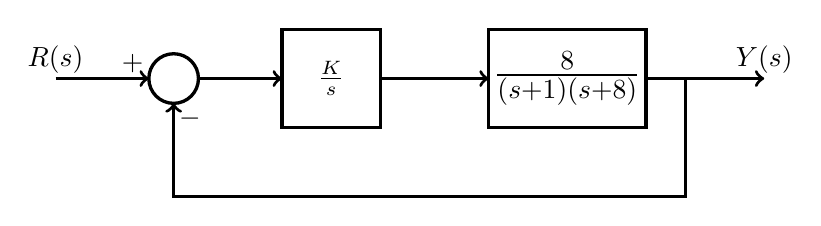
\begin{tikzpicture}[scale=1,inner sep=0pt,outer sep=0pt,very thick,
sysblock/.style={draw,rectangle,inner sep=2pt,minimum width=1.25cm,minimum height=1.25cm,very thick}]
\draw (2,0) node[draw,circle] (sum1) {$\rule{0pt}{18pt}$};
\draw (4,0) node[sysblock] (Kp) {$\frac{K}{s}$};
\draw (7,0) node[sysblock] (G) {\Large$\frac{8}{(s+1)(s+8)}$};
\draw[->] (.5,0) node[above=2pt] {$R(s)$} -- (sum1.180) node[above left=2pt] {$+$};
\draw[->] (sum1.0) --  (Kp);
\draw[->] (Kp) -- (G.180);
\draw[->] (G) -- ++(2.5,0) node[above=2pt] {$Y(s)$};
\draw[->] (G) ++(1.5,0) -- ++(0,-1.5) -| (sum1.-90) node[below right=2pt] {$-$};
\end{tikzpicture}


\begin{enumerate}[(a)]
\item Derive the transfer function from the reference $r(t)$ to the reference error $e(t)$.
\item Find the feasible range for the parameter $K$ so that the system is stable.
\item Calculate the steady-state error with respect to a unit ramp input $r(t)=tu(t)$.  
\item What value of $K$ minimizes the error and what is the value of the error?
\end{enumerate}


\end{center}


